\ifx\allfiles\undefined
\documentclass[12pt, a4paper,oneside, UTF8]{ctexbook}
\usepackage[dvipsnames]{xcolor}
\usepackage{amsmath}   % 数学公式
\usepackage{amsthm}    % 定理环境
\usepackage{amssymb}   % 更多公式符号
\usepackage{graphicx}  % 插图
%\usepackage{mathrsfs}  % 数学字体
%\usepackage{newtxtext,newtxmath}
%\usepackage{arev}
\usepackage{kmath,kerkis}
\usepackage{newtxtext}
\usepackage{bbm}
\usepackage{enumitem}  % 列表
\usepackage{geometry}  % 页面调整
%\usepackage{unicode-math}
\usepackage[colorlinks,linkcolor=black]{hyperref}

\usepackage{wrapfig}


\usepackage{ulem}	   % 用于更多的下划线格式,
					   % \uline{}下划线,\uuline{}双下划线,\uwave{}下划波浪线,\sout{}中间删除线,\xout{}斜删除线
					   % \dashuline{}下划虚线,\dotuline{}文字底部加点


\graphicspath{ {flg/},{../flg/}, {config/}, {../config/} }  % 配置图形文件检索目录
\linespread{1.5} % 行高

% 页码设置
\geometry{top=25.4mm,bottom=25.4mm,left=20mm,right=20mm,headheight=2.17cm,headsep=4mm,footskip=12mm}

% 设置列表环境的上下间距
\setenumerate[1]{itemsep=5pt,partopsep=0pt,parsep=\parskip,topsep=5pt}
\setitemize[1]{itemsep=5pt,partopsep=0pt,parsep=\parskip,topsep=5pt}
\setdescription{itemsep=5pt,partopsep=0pt,parsep=\parskip,topsep=5pt}

% 定理环境
% ########## 定理环境 start ####################################
\theoremstyle{definition}
\newtheorem{defn}{\indent 定义}[section]

\newtheorem{lemma}{\indent 引理}[section]    % 引理 定理 推论 准则 共用一个编号计数
\newtheorem{thm}[lemma]{\indent 定理}
\newtheorem{corollary}[lemma]{\indent 推论}
\newtheorem{criterion}[lemma]{\indent 准则}

\newtheorem{proposition}{\indent 命题}[section]
\newtheorem{example}{\indent \color{SeaGreen}{例}}[section] % 绿色文字的 例 ,不需要就去除\color{SeaGreen}{}
\newtheorem*{rmk}{\indent \color{red}{注}}

% 两种方式定义中文的 证明 和 解 的环境:
% 缺点:\qedhere 命令将会失效【技术有限,暂时无法解决】
\renewenvironment{proof}{\par\textbf{证明.}\;}{\qed\par}
\newenvironment{solution}{\par{\textbf{解.}}\;}{\qed\par}

% 缺点:\bf 是过时命令,可以用 textb f等替代,但编译会有关于字体的警告,不过不影响使用【技术有限,暂时无法解决】
%\renewcommand{\proofname}{\indent\bf 证明}
%\newenvironment{solution}{\begin{proof}[\indent\bf 解]}{\end{proof}}
% ######### 定理环境 end  #####################################

% ↓↓↓↓↓↓↓↓↓↓↓↓↓↓↓↓↓ 以下是自定义的命令  ↓↓↓↓↓↓↓↓↓↓↓↓↓↓↓↓

% 用于调整表格的高度  使用 \hline\xrowht{25pt}
\newcommand{\xrowht}[2][0]{\addstackgap[.5\dimexpr#2\relax]{\vphantom{#1}}}

% 表格环境内长内容换行
\newcommand{\tabincell}[2]{\begin{tabular}{@{}#1@{}}#2\end{tabular}}

% 使用\linespread{1.5} 之后 cases 环境的行高也会改变,重新定义一个 ca 环境可以自动控制 cases 环境行高
\newenvironment{ca}[1][1]{\linespread{#1} \selectfont \begin{cases}}{\end{cases}}
% 和上面一样
\newenvironment{vx}[1][1]{\linespread{#1} \selectfont \begin{vmatrix}}{\end{vmatrix}}

\def\d{\textup{d}} % 直立体 d 用于微分符号 dx
\def\R{\mathbb{R}} % 实数域
\def\N{\mathbb{N}} % 自然数域
\def\C{\mathbb{C}} % 复数域
\def\Z{\mathbb{Z}} % 整数环
\def\Q{\mathbb{Q}} % 有理数域
\newcommand{\bs}[1]{\boldsymbol{#1}}    % 加粗,常用于向量
\newcommand{\ora}[1]{\overrightarrow{#1}} % 向量

% 数学 平行 符号
\newcommand{\pll}{\kern 0.56em/\kern -0.8em /\kern 0.56em}

% 用于空行\myspace{1} 表示空一行 填 2 表示空两行  
\newcommand{\myspace}[1]{\par\vspace{#1\baselineskip}}

%s.t. 用\st就能打出s.t.
\DeclareMathOperator{\st}{s.t.}

%罗马数字 \rmnum{}是小写罗马数字, \Rmnum{}是大写罗马数字
\makeatletter
\newcommand{\rmnum}[1]{\romannumeral #1}
\newcommand{\Rmnum}[1]{\expandafter@slowromancap\romannumeral #1@}
\makeatother
\begin{document}
	% \title{{\Huge{\textbf{$Real \,\, Analysis$}}}\\
		\Large{\textbf{$Measure \,\, Theory , \,\, Integration , \,\, \& \,\, Hilbert \,\, Spaces$}}\footnote{参考书籍:\\
			\hspace*{4em} \textbf{《$Real \,\, Analysis -- Measure \,\, Theroy, \,\, Integration, \,\, \& \,\, Hilbert \,\, Spaces$》--- $Elias \,\, M. \,\, Stein$} \\
			\hspace*{4em} \textbf{《$Real \,\, Analysis -- Modern \,\, Techniques \,\, and \,\, Their \,\, Applications$》--- $Gerald \,\, B. \,\, Folland$}}}
\author{$-TW-$}
\date{\today}
\maketitle                   % 在单独的标题页上生成一个标题

\thispagestyle{empty}        % 前言页面不使用页码
\begin{center}
	\Huge\textbf{序}
\end{center}


\vspace*{3em}
\begin{center}
	\large{\textbf{天道几何,万品流形先自守;}}\\
	
	\large{\textbf{变分无限,孤心测度有同伦。}}
\end{center}

\vspace*{3em}
\begin{flushright}
	\begin{tabular}{c}
		\today \\ \small{\textbf{长夜伴浪破晓梦,梦晓破浪伴夜长}}
	\end{tabular}
\end{flushright}


\newpage                      % 新的一页
\pagestyle{plain}             % 设置页眉和页脚的排版方式(plain:页眉是空的,页脚只包含一个居中的页码)
\setcounter{page}{1}          % 重新定义页码从第一页开始
\pagenumbering{Roman}         % 使用大写的罗马数字作为页码
\tableofcontents              % 生成目录

\newpage                      % 以下是正文
\pagestyle{plain}
\setcounter{page}{1}          % 使用阿拉伯数字作为页码
\pagenumbering{arabic}
\setcounter{chapter}{0}    % 设置 -1 可作为第零章绪论从第零章开始 
	\else
	\fi
	%  ############################ 正文部分
\chapter{$Measures$}

\newpage
\setcounter{section}{3}
\section{$Outer \,\, Measures$}
	\begin{proposition}\label{prop 2.4.1}
		Let $\mathcal{E} \subset \mathcal{P}(X)$ and $\rho : \mathcal{E} \rightarrow [0 , \infty]$ be such that $\varnothing \in \mathcal{E}$, $X \in \mathcal{E}$ and $\rho(\varnothing) = 0$. For any $A \subset X$, define
		\begin{align}
			\mu^{*}(A) = \inf{\left\{ \sum_{j = 1}^{\infty}{\rho(E_j)} \mid E_j \in \mathcal{E} \,\, and \,\, A \subset \bigcup_{j = 1}^{\infty}{E_j} \right\}}
		\end{align}
		Then $\mu^{*}$ is an outer measure.
	\end{proposition}
	
	\vspace*{10em}
	
	\begin{thm}\label{thm 2.4.1}
		\textbf{Carath\'{e}odory's Theorem}. \\
		If $\mu^{*}$ is an outer measure on $X$, the collection $\mathcal{M}$ of $\mu^{*}$-measurable sets is a $\sigma$-algebra, and the restriction of $\mu^{*}$ to $\mathcal{M}$ is a complete measure.
	\end{thm}
	
	\vspace*{10em}
	
	\begin{proposition}\label{prop 2.4.2}
		If $\mu_0$ is a premeasure on $\mathcal{A}$ and $\mu^{*}$ is an outer measure defined by
		\begin{align}
			\mu^{*}(E) = \inf{\left\{ \sum_{j = 1}^{\infty}{\rho(A_j)} \mid A_j \in \mathcal{A} \,\, and \,\, E \subset \bigcup_{j = 1}^{\infty}{A_j} \right\}}
		\end{align}
		then
		\begin{enumerate}
			\item[a.] $\mu^{*} \mid_\mathcal{A} = \mu_0$;
			
			\item[b.] Every set in $\mathcal{A}$ is $\mu^{*}$-measurable.
		\end{enumerate}
	\end{proposition}
	
	\newpage
	
	\begin{thm}\label{thm 2.4.2}
		Let $\mathcal{A} \subset \mathcal{P}(X)$ be an algebra, $\mu_0$ a premeasure on $\mathcal{A}$, and $\mathcal{M}$ the $\sigma$-algebra generated by $\mathcal{A}$. There exists a measure $\mu$ on $\mathcal{M}$ whose restriction to $\mathcal{A}$ is $\mu_0$ -- namely, $\mu = \mu^{*} \mid_{\mathcal{M}}$ where $\mu^{*}$ is given by 
		\begin{align}
			\mu^{*}(E) = \inf{\left\{ \sum_{j = 1}^{\infty}{\rho(A_j)} \mid A_j \in \mathcal{A} \,\, and \,\, E \subset \bigcup_{j = 1}^{\infty}{A_j} \right\}}
		\end{align}
		If $\nu$ is another measure on $\mathcal{M}$ that extends $\mu_0$, then
		\begin{align}
			\nu(E) \leq \mu(E) , \,\, \forall E \in \mathcal{M}
		\end{align}
		with equality when $\mu(E) < \infty$.\\
		If $\mu_0$ is $\sigma$-finite, then $\mu$ is the unique extension of $\mu_0$ to a measure on $\mathcal{M}$.
	\end{thm}

\newpage

\section{$Borel \,\, Measures \,\, on \,\, the \,\, Real \,\, Line$}
	\begin{proposition}\label{prop 2.5.1}
		Let $F : \R \rightarrow \R$ be increasing and right continuous. If $(a_j , b_j] , j = 1 \sim n$ are disjoint h-intervals, let
		\begin{align}
			\mu_0(\bigcup_{j = 1}^{n}{(a_j , b_j]}) = \sum_{j = 1}^{n}{\left[ F(b_j) - F(a_j) \right]}
		\end{align}
		and let $\mu_0(\varnothing) = 0$. Then $\mu_0$ is a premeasure on the algebra $\mathcal{A}$, where
		\begin{align}
			\mathcal{A} = \left\{ finite \,\, disjoint \,\, unions \,\, of \,\, h-intervals \right\}
		\end{align}
	\end{proposition}
	
	\vspace*{16em}
	
	\begin{thm}\label{thm 2.5.1}
		If $F : \R \rightarrow \R$ is any increasing, right continuous function, there is a unique Borel measure $\mu_F$ on $\R$ such that 
		\begin{align}
			\mu_F((a , b]) = F(b) - F(a) , \,\, \forall a , b
		\end{align}
		If $G$ is another such function, we have
		\begin{center}
			$\mu_F = \mu_G \,\, \Leftrightarrow \,\, F - G$ is constant
		\end{center}
		Conversely, if $\mu$ is a Borel measure on $\R$ that is finite on all bounded Borel sets and we define
		\begin{align}
			F(x) = 
			\begin{cases}
				\mu((0 , x]) , \,\, if \,\, x > 0 \\
				0 , \,\, if \,\, x = 0 \\
				-\mu((x , 0]) , \,\, if \,\, x < 0
			\end{cases}
		\end{align}
		then $F$ is increasing and right continuous, and $\mu = \mu_F$.
	\end{thm}

	\newpage
	
	\begin{lemma}\label{lemma 2.5.2}
		Fix a complete Lebesgue-Stieltjes measure $\mu$ on $\R$ associated to the increasing, right continuous function $F$, and we denote by $\mathcal{M}_\mu$ the domain of $\mu$ ($\mathcal{M}_\mu$ is always strictly larger than $\mathcal{B}_\R$). Then for any $E \in \mathcal{M}_\mu$,
		\begin{align}
			\mu(E) 
			&= \inf{\left\{ \sum_{j = 1}^{\infty}{\left[ F(b_j) - F(a_j) \right]} \mid E \subset \bigcup_{j = 1}^{\infty}{(a_j , b_j]} \right\}} \\
			&= \inf{\left\{ \sum_{j = 1}^{\infty}{\mu((a_j , b_j])} \mid E \subset \bigcup_{j = 1}^{\infty}{(a_j , b_j]} \right\}} \\
			&= \inf{\left\{ \sum_{j = 1}^{\infty}{\mu((a_j , b_j))} \mid E \subset \bigcup_{j = 1}^{\infty}{(a_j , b_j)} \right\}}
		\end{align}
	\end{lemma}
	
	\vspace*{6em}
	
	\begin{thm}\label{thm 2.5.3}
		If $E \in \mathcal{M}_\mu$, then
		\begin{align}
			\mu(E) 
			&= \inf{\left\{ \mu(U) \mid E \subset U \,\, and \,\, U \,\, is \,\, open \right\}} \\
			&= \sup{\left\{ \mu(K) \mid K \subset E \,\, and \,\, K \,\, is \,\, compact \right\}}
		\end{align}
	\end{thm}
	
	\vspace*{6em}
	
	\begin{thm}\label{thm 2.5.4}
		\textbf{正则性}. \\
		If $E \subset \R$, the followings are equivalent:
		\begin{enumerate}
			\item[a.] $E \in \mathcal{M_\mu}$.
			
			\item[b.] $E = V \backslash N_1$ where $V$ is a $G_\delta$ set and $\mu(N_1) = 0$. 
			
			\item[c.] $E = H \cup N_2$ where $H$ is an $F_\sigma$ det and $\mu(N_2) = 0$.
		\end{enumerate}
	\end{thm}

	\vspace*{6em}
	
	\begin{proposition}\label{prop 2.5.2}
		If $E \in \mathcal{M}_\mu$ and $\mu(E) < \infty$, then $\forall \epsilon > 0$, $\exists A = $ finite disjoint union of open intervals, $\st$
		\begin{align}
			\mu(E \triangle A) < \epsilon
		\end{align}
	\end{proposition}
	
	\newpage
	
	\begin{thm}\label{thm 2.5.5}
		If $E \in \mathcal{L}$, then
		\begin{align}
			E + s \in \mathcal{L} \,\, and \,\, rE \in \mathcal{L} , \,\, \forall s , r \in \R
		\end{align}
		Moreover, 
		\begin{align}
			m(E + s) = m(E) \,\, and \,\, m(rE) = \left| r \right| m(E)
		\end{align}
	\end{thm}
	
	\vspace*{20em}
	
	\begin{proposition}\label{prop 2.5.3}
		Let $C$ be the Cantor set.
		
		\vspace*{1em}
		\begin{enumerate}
			\item[a.] $C$ is compact, nowhere dense, and totally disconnected.
			\begin{center}
				(i.e. the only connected subset of $C$ are single points)
			\end{center}
			Moreover, $C$ has no isolated points.
			
			\vspace*{1em}
			
			\item[b.] $m(C) = 0$. 
			
			\vspace*{1em}
			
			\item[c.] $card(C) = \aleph$.
		\end{enumerate}
	\end{proposition}
	
	\newpage
	
	\begin{figure}[thbp!]
		\centering
		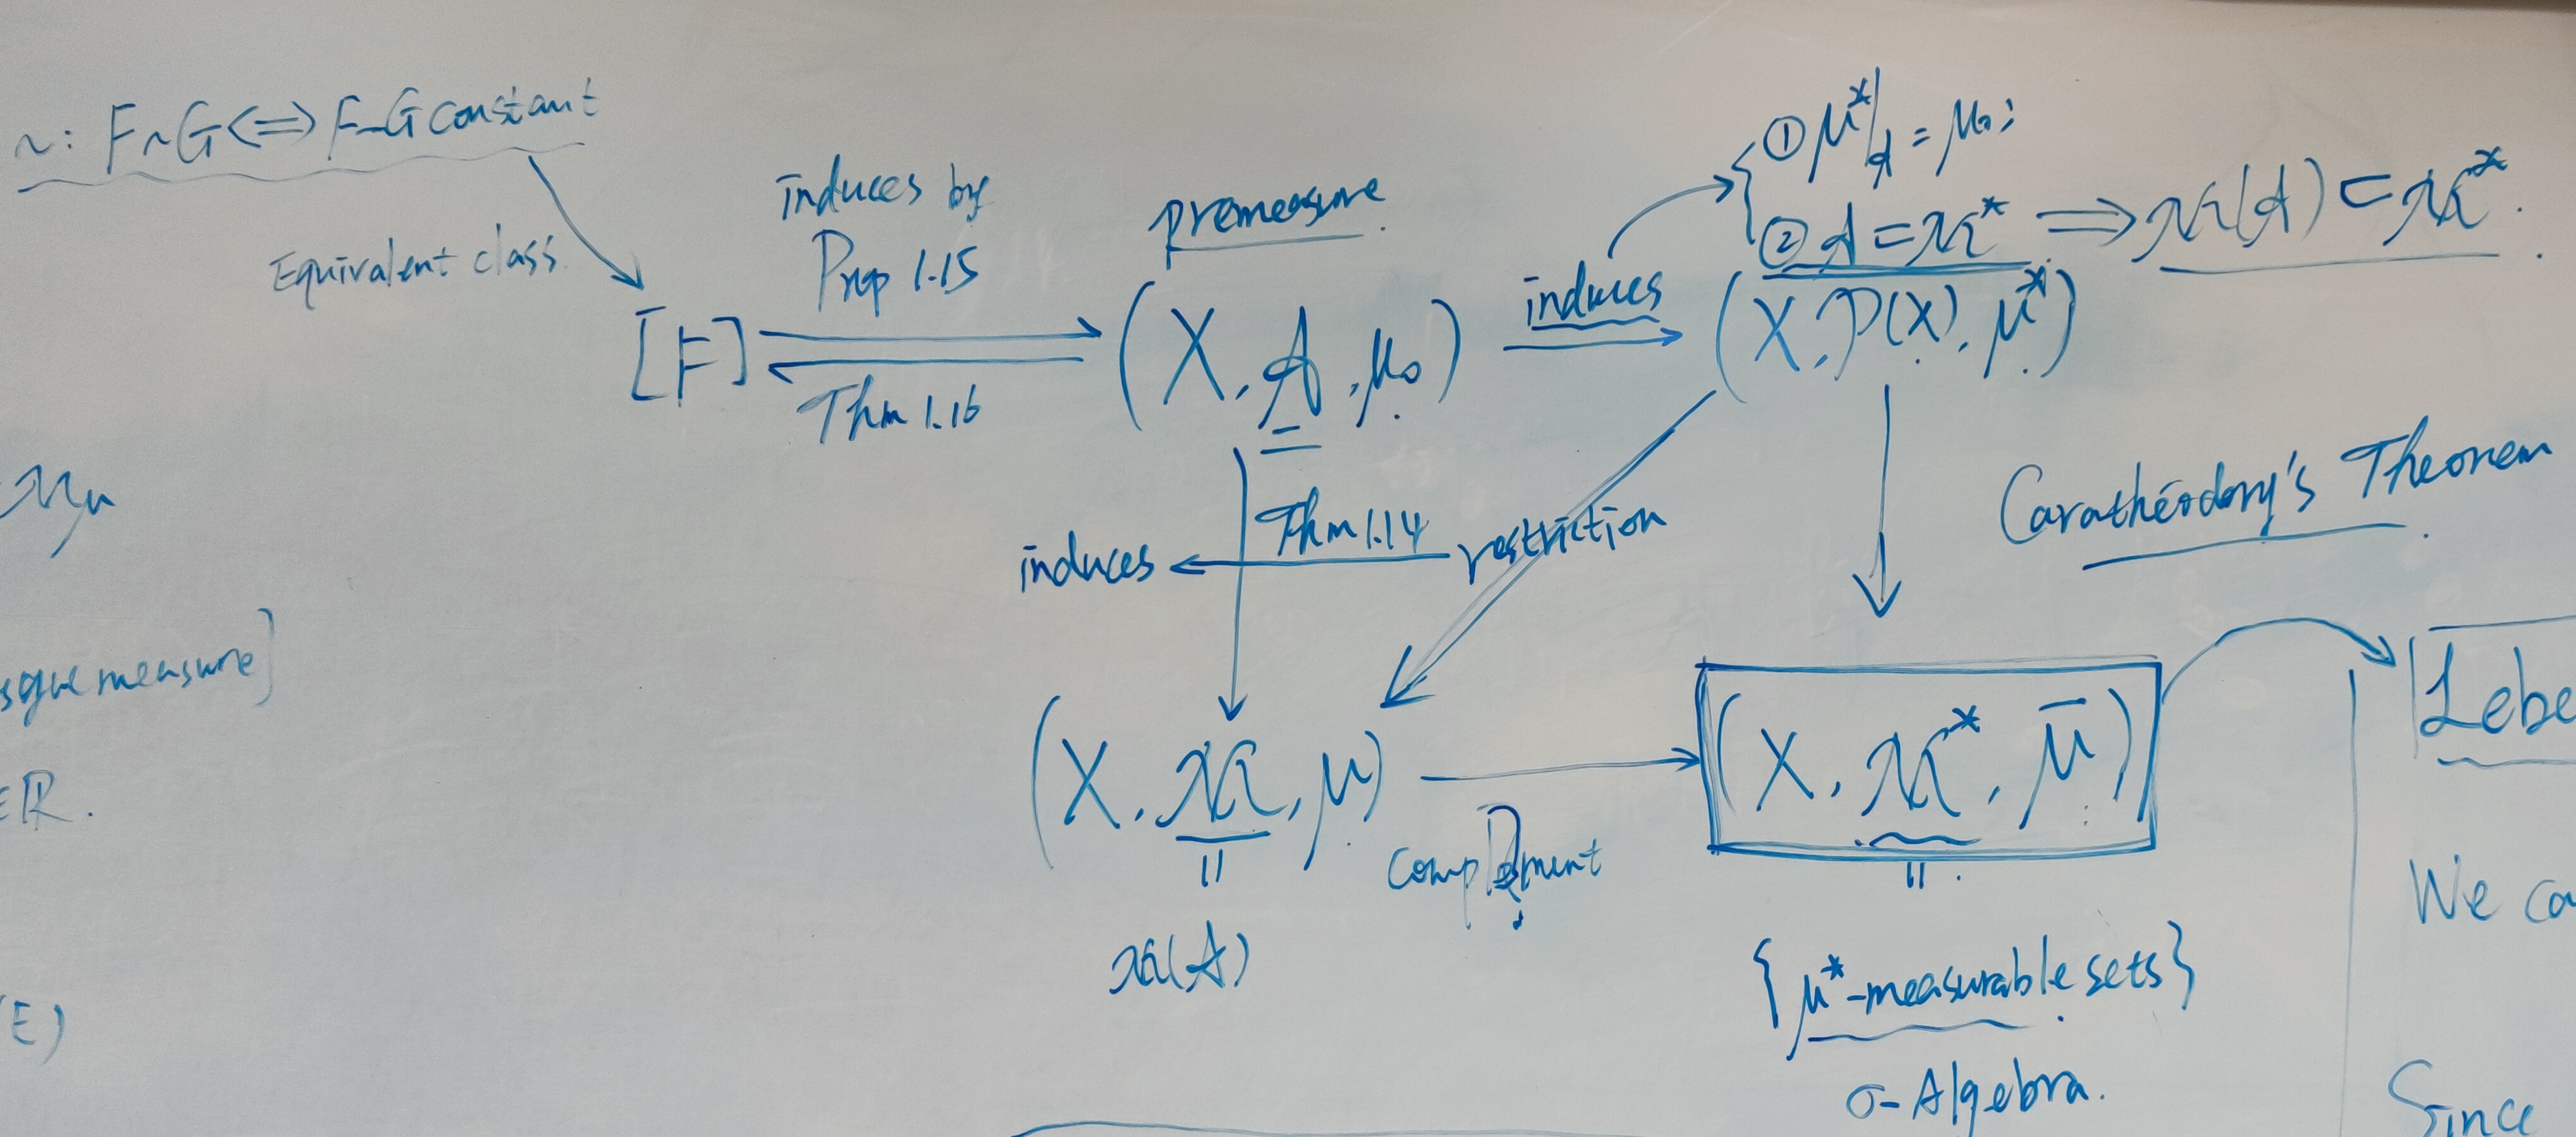
\includegraphics[width=1.0\linewidth]{figure/1.5}
		\caption{Measure Theory}
		\label{pic : 4.7.2-1} % 添加图像引用标签
	\end{figure}

	%  ############################
	\ifx\allfiles\undefined
\end{document}
\fi